\documentclass{article}
\usepackage[utf8]{inputenc}
\usepackage{graphicx}
\usepackage{wrapfig}
\usepackage[left=1in, right=1in, top=.5in]{geometry}
\usepackage{subfig}
\usepackage{enumitem}

\graphicspath{ {./images/} }

\title{6.867}
\author{anonymous}
\date{September 2018}

\begin{document}
\maketitle

\section{Part 1}
Didn't have time to do nice Latex equations (or even the fourth problem) so please pardon the pasted in pics of some of the more mathy solutions :) 
\begin{enumerate}[label=\alph*.)]
	\item  Bayes classifier and error:\\
	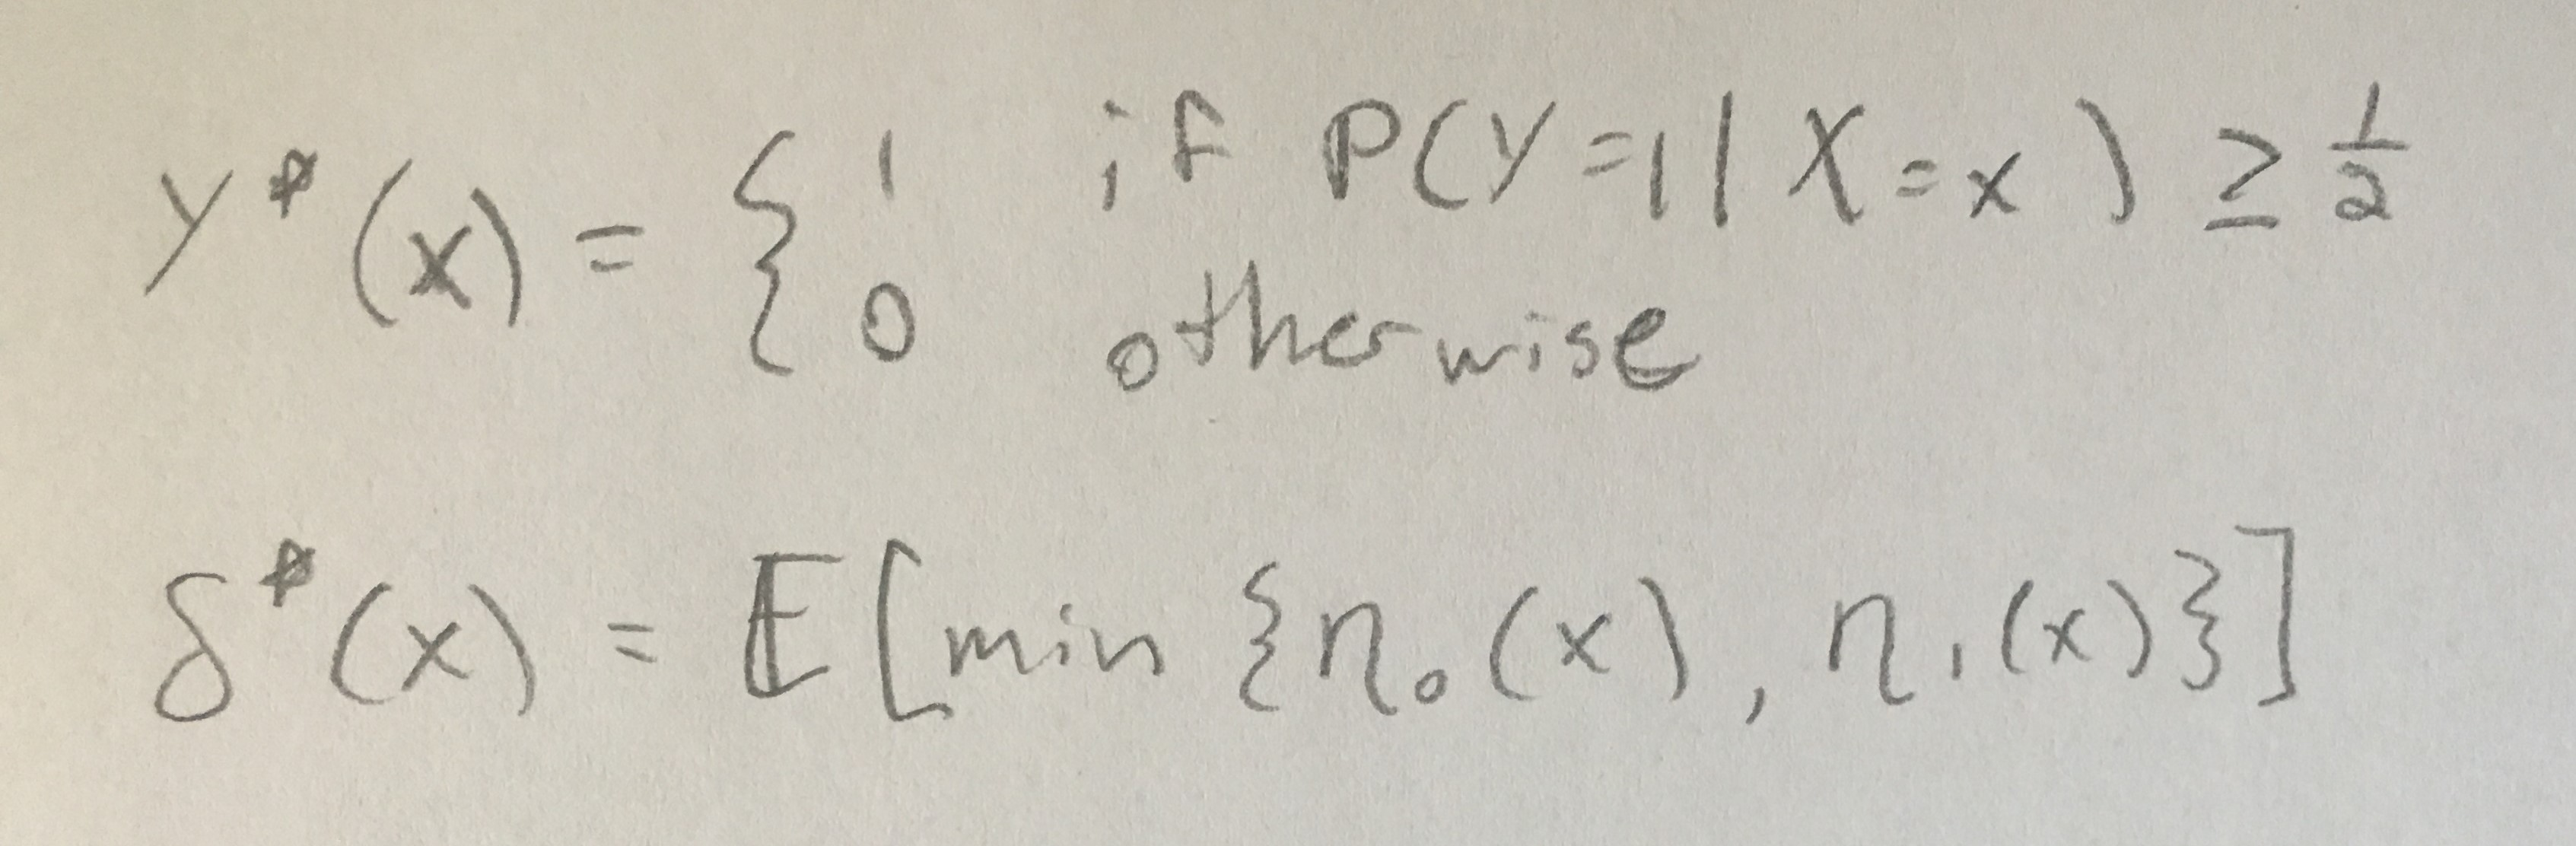
\includegraphics[scale=.05]{IMG_3677.JPG}
	\item We know that the 1-NN algorithm has a VC dimension which goes to infinity because it is capable of shattering any number of points. This is because, if we take a set of points in continuous space which are not overlapping, then regardless of the points' labels we can classify them correctly by placing the same set of points as the testing set. This means that a model has the potential to over fit to testing data in the greatest possible extreme, thus generalization error has the potential to be very high.  
	\item Since the variables are identically and independently distributed, this limit is equal to the probability that any one of the training points is greater than beta and raised to the power of n. And since there is a nonzero chance that a training point is within a non-zero distance of the testing point, we know that the there is a less than 1 chance that a given training point is outside this range. Thus a less-than-one chance raised to the power of n approaches zero as n goes to infinity. Symbolically: \\
	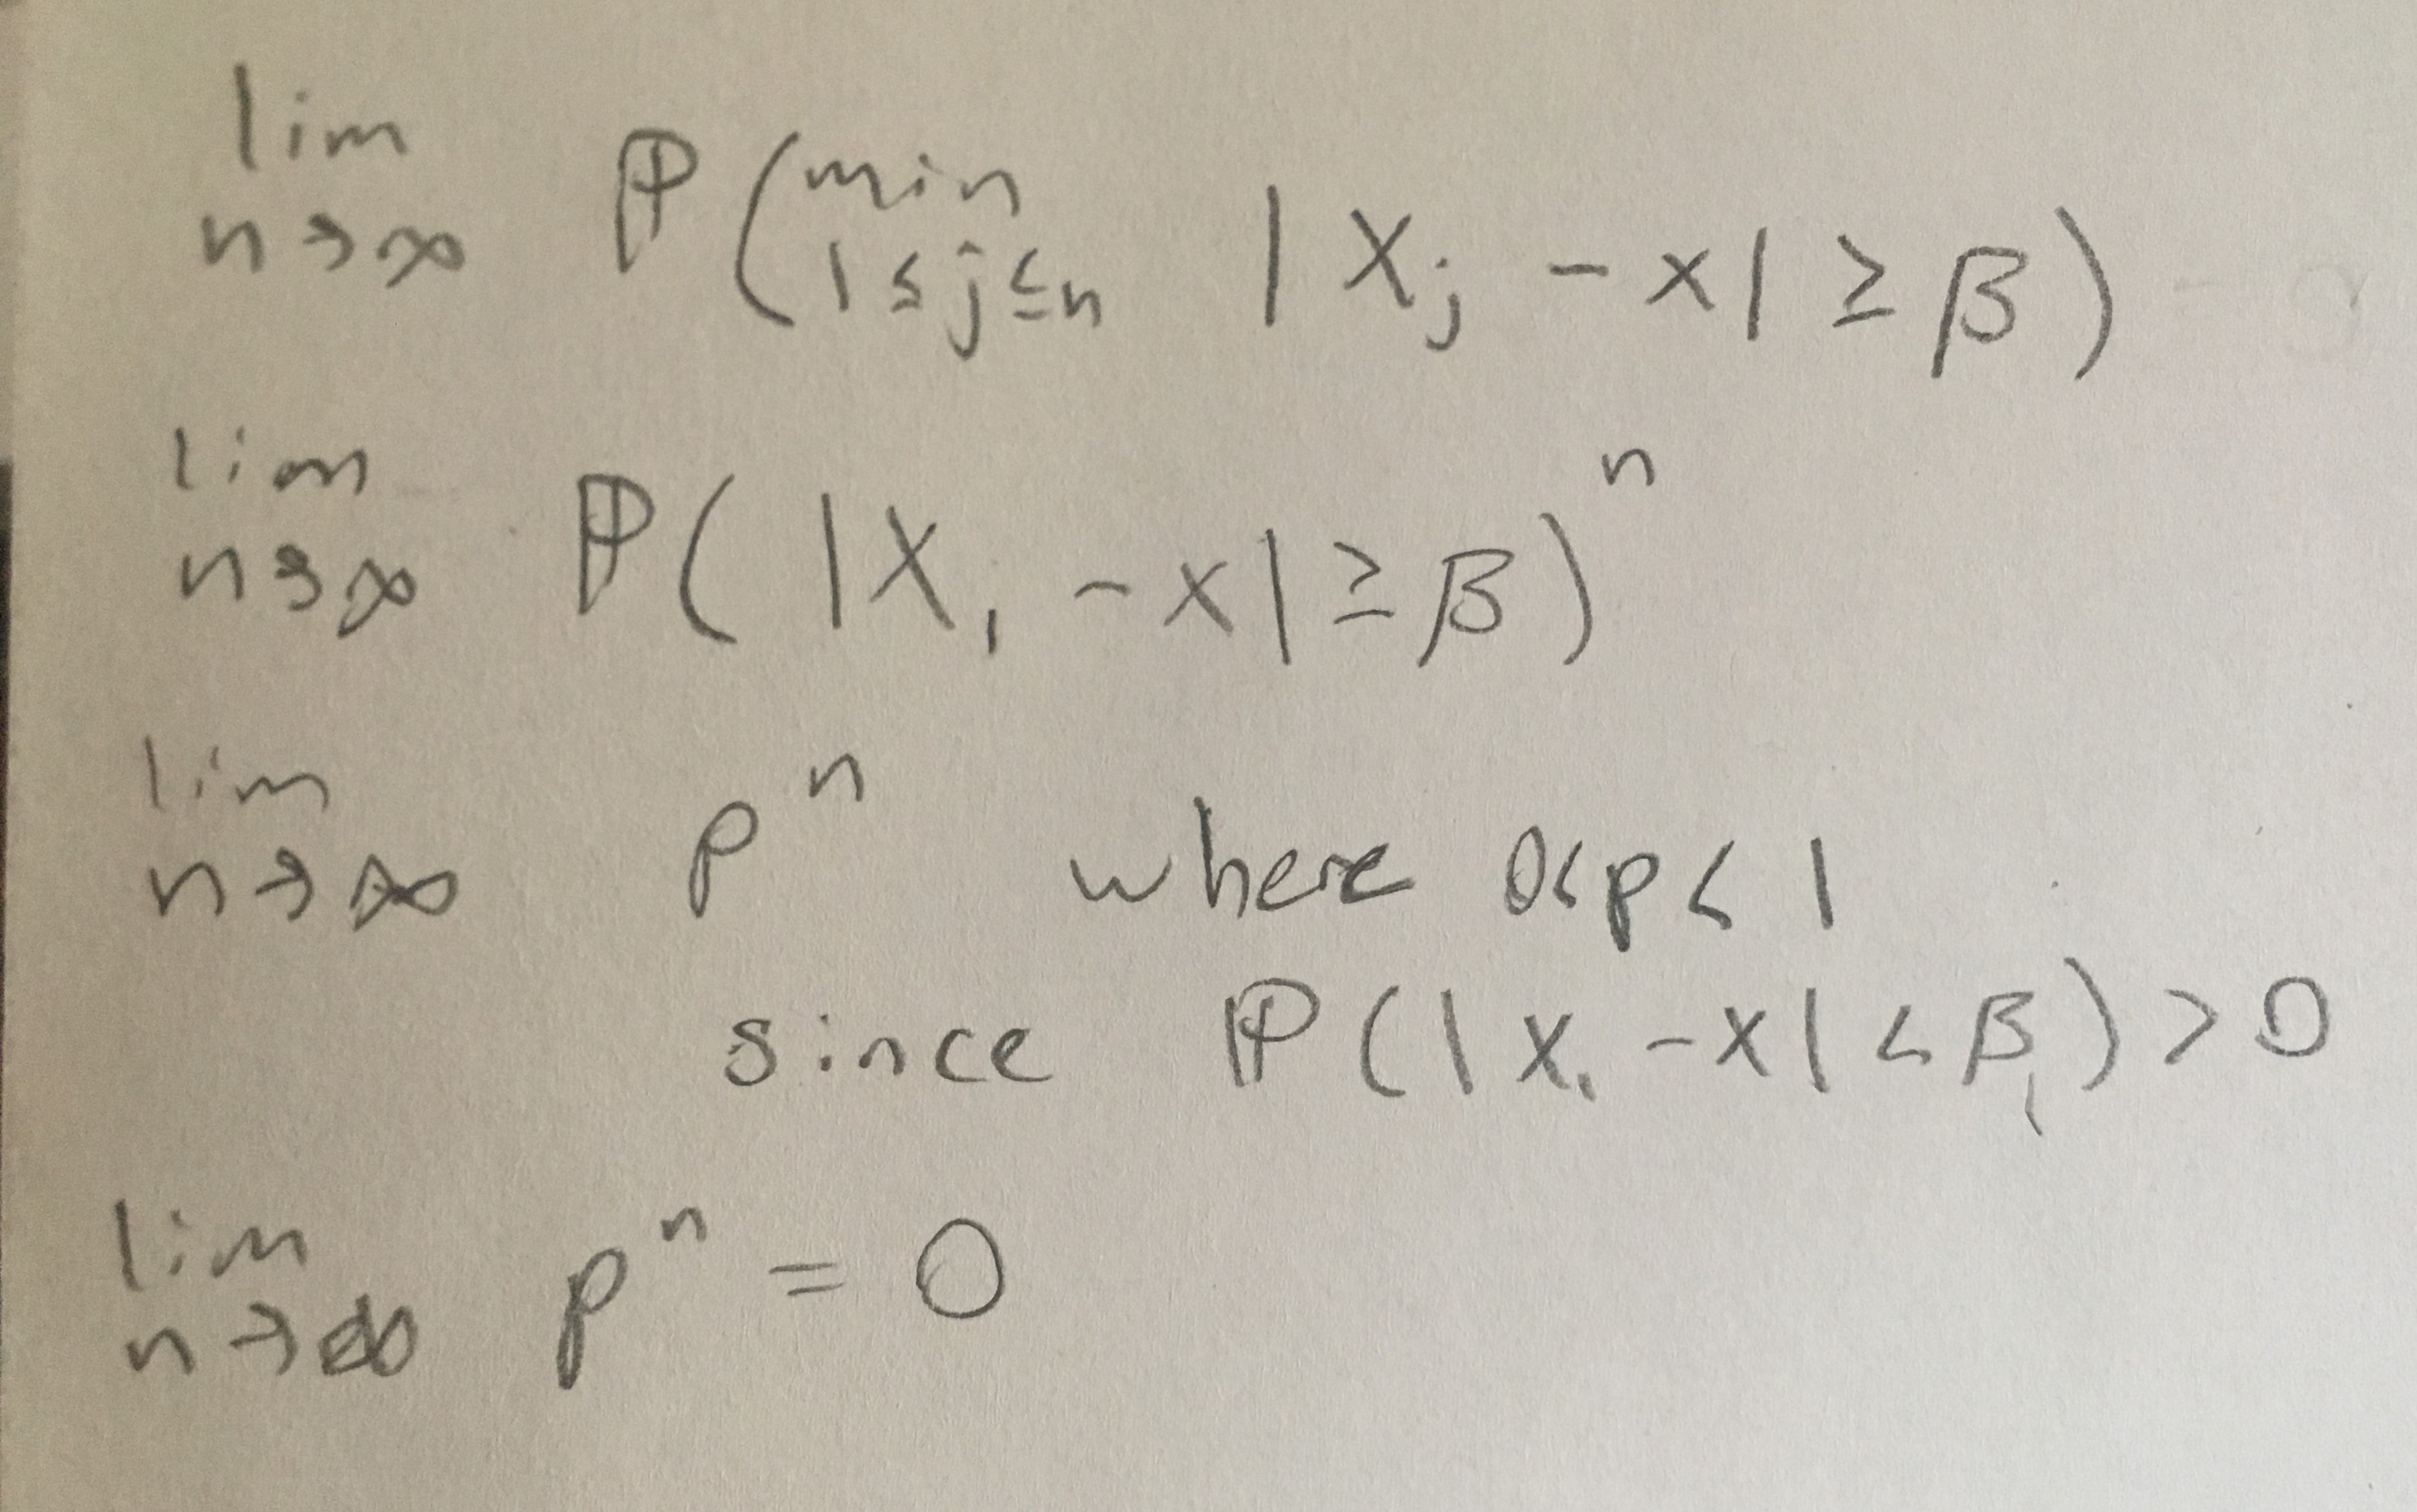
\includegraphics[scale=.05]{IMG_3678.JPG}
	\item The probability that the prediction is wrong given an x for a binary classification problem is simply the chance that it predicts a 1 when it should be a 0 or predicts a 0 when it should be a 1. More rigorously, this is the probability that the true class is 0 given x times the probability that the model will predict a 1 given x all plus the the probability that the true class is 1 given x times the probability that the model will predict a 0 given x. Symbolically, this means:\\
	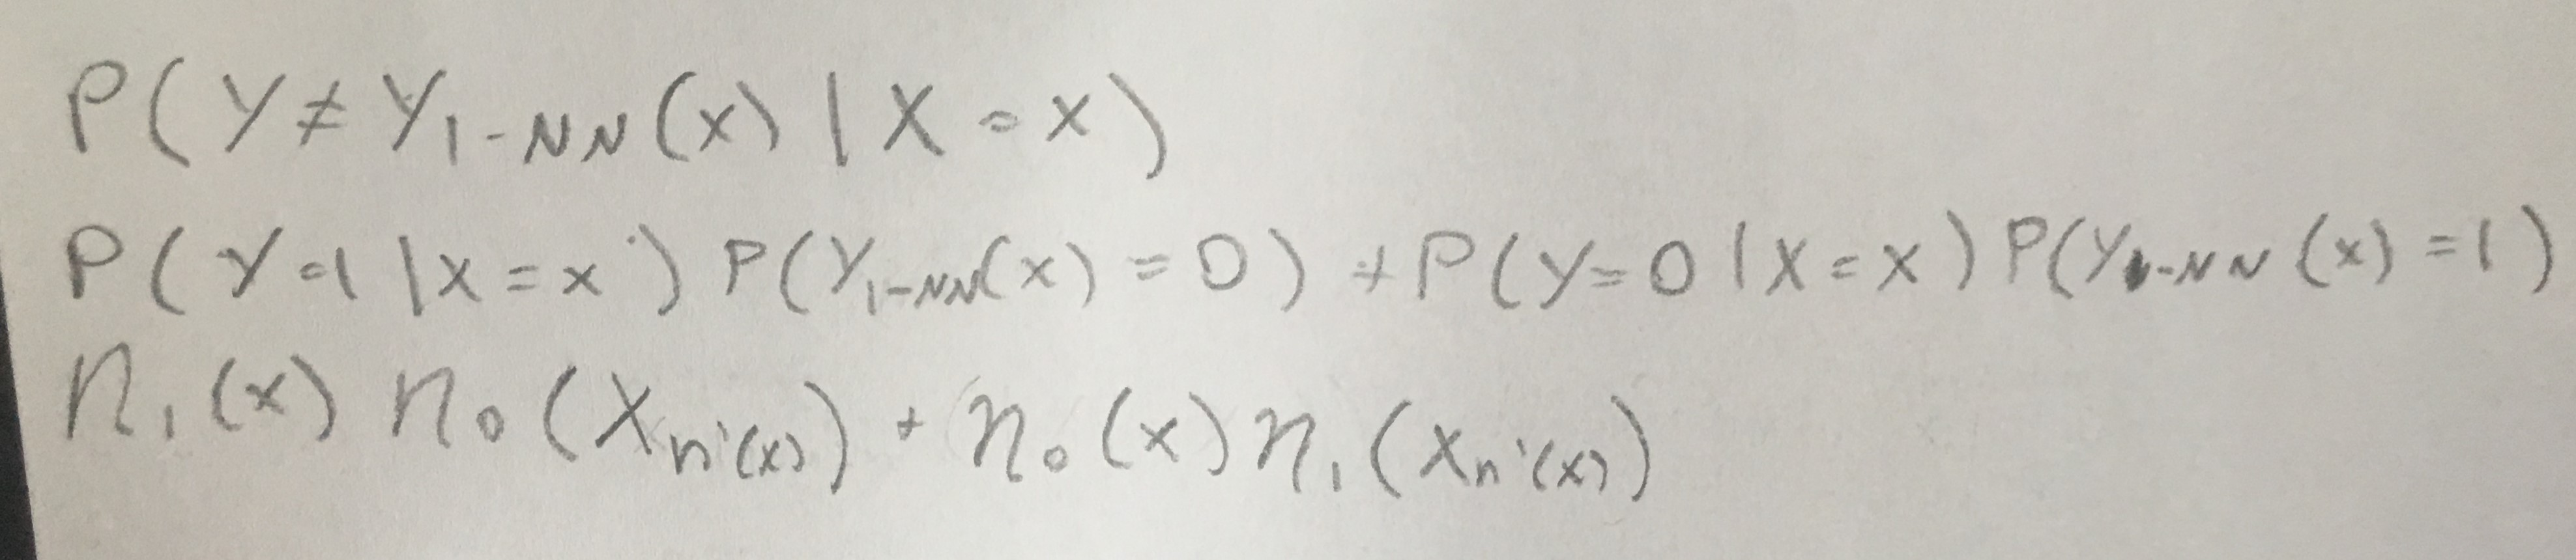
\includegraphics[scale=.075]{IMG_3679.JPG}\\
	The limit of the probability that the closest point to a given point x is a class c simply approaches the probability that the same given point x is in the class c. This is because, as shown in part c, as we get more training points, the probability that none of them are within a certain distance of a given testing point x goes to zero, the contrapositive being that the probability approaches one that there is already at least one point where the test point x is. That means that, since the point (or set of points) at x as n goes to infinity are the same as x, they must by definition have the same conditional distribution. Symbolically, this means:\\
	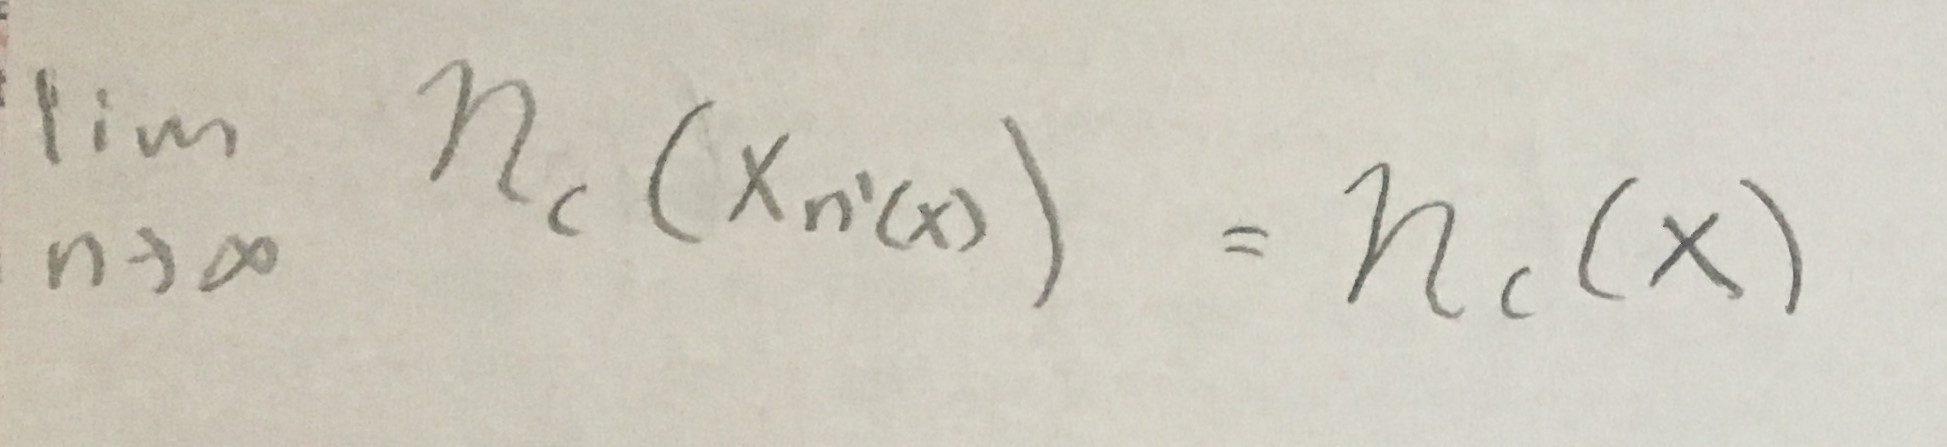
\includegraphics[scale=.15]{IMG_3683.JPG}
	\item Given a particular x, the definition of the Bayes error simply becomes the minimum of the probabilities that x is of either class (since, given a particular x, an expectation conditional on that x disappears). By part d, the limit as n goes to infinity of the probability of classification just goes to two times the conditional probability of class 0 times the conditional probability of class 1. Symbolically, we can see how this proves the inequality that the probability of KNN-1 misclassification goes to two times the probability of Bayes Error. \\
	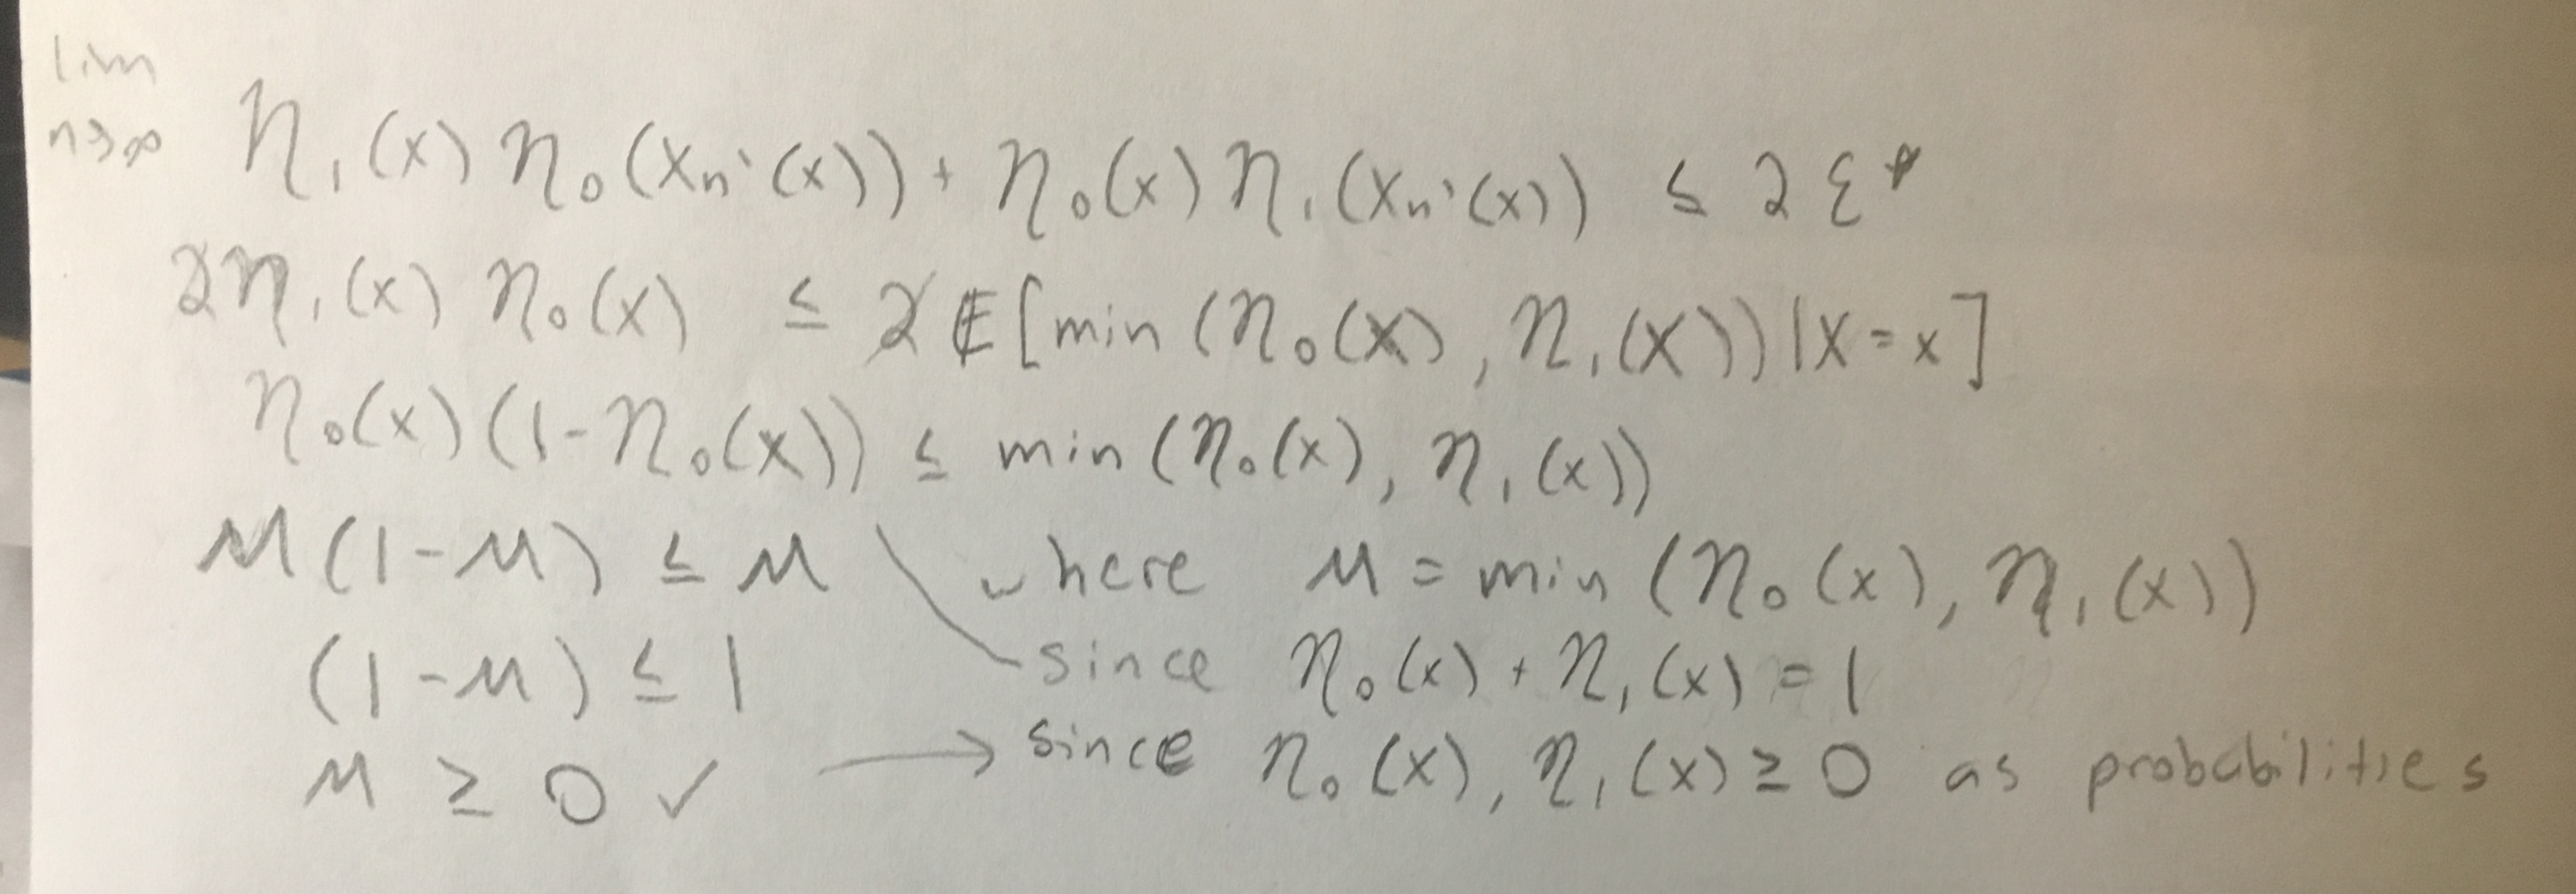
\includegraphics[scale=.1]{IMG_3688.jpg}
\end{enumerate}


\section{Part 2}
\begin{enumerate}
\item 

\begin{enumerate}
\item if we take the standard basis for d-space of d independent unit vectors, each with a single non-zero dimension, then we can see that a hyperplane can shatter any labelling of these points. this is because, for any labelling of the vectors, we can let the hyperplane normal have the same value as the class (where the possible classes are 1 and -1). This means that for a basis vector with a -1 in the ith position, the hyperplane normal will also have a -1 in the ith position, thus the inner product with that vector is 1 and that vector will be correctly classified.  Since all vectors are ind pendent and only have one nonzero term each and there are d of them, we know there is a bijective mapping between dimensions on the hyperplane normal and vectors which are nonzero along that dimension. In other words, the hyperplane will be completely defined by the classes of the basis vectors. This also means every basis vector will be correctly classified. Thus the set is shattered and VC $\geq$ d.\\
\item for any set of d+1 vectors in d space we know that this set of vectors is not independent (since there can be at most d independent vectors in d space). Therefore we can choose one vector $x_0$ to solve for as a linear combination of the other d vectors (ie as a weighted sum of the other vectors). If we multiply both sides by the hyperplane normal w, we see that the this weighted sum times w becomes the same as the weighted sum (with the same coefficients) of the other d vectors' classifications, which means the classification w times $x_0$ is deterministic in the context of the classifications of the other d vectors, regardless of $x_0$'s true class. Symbolically, we can show: \\
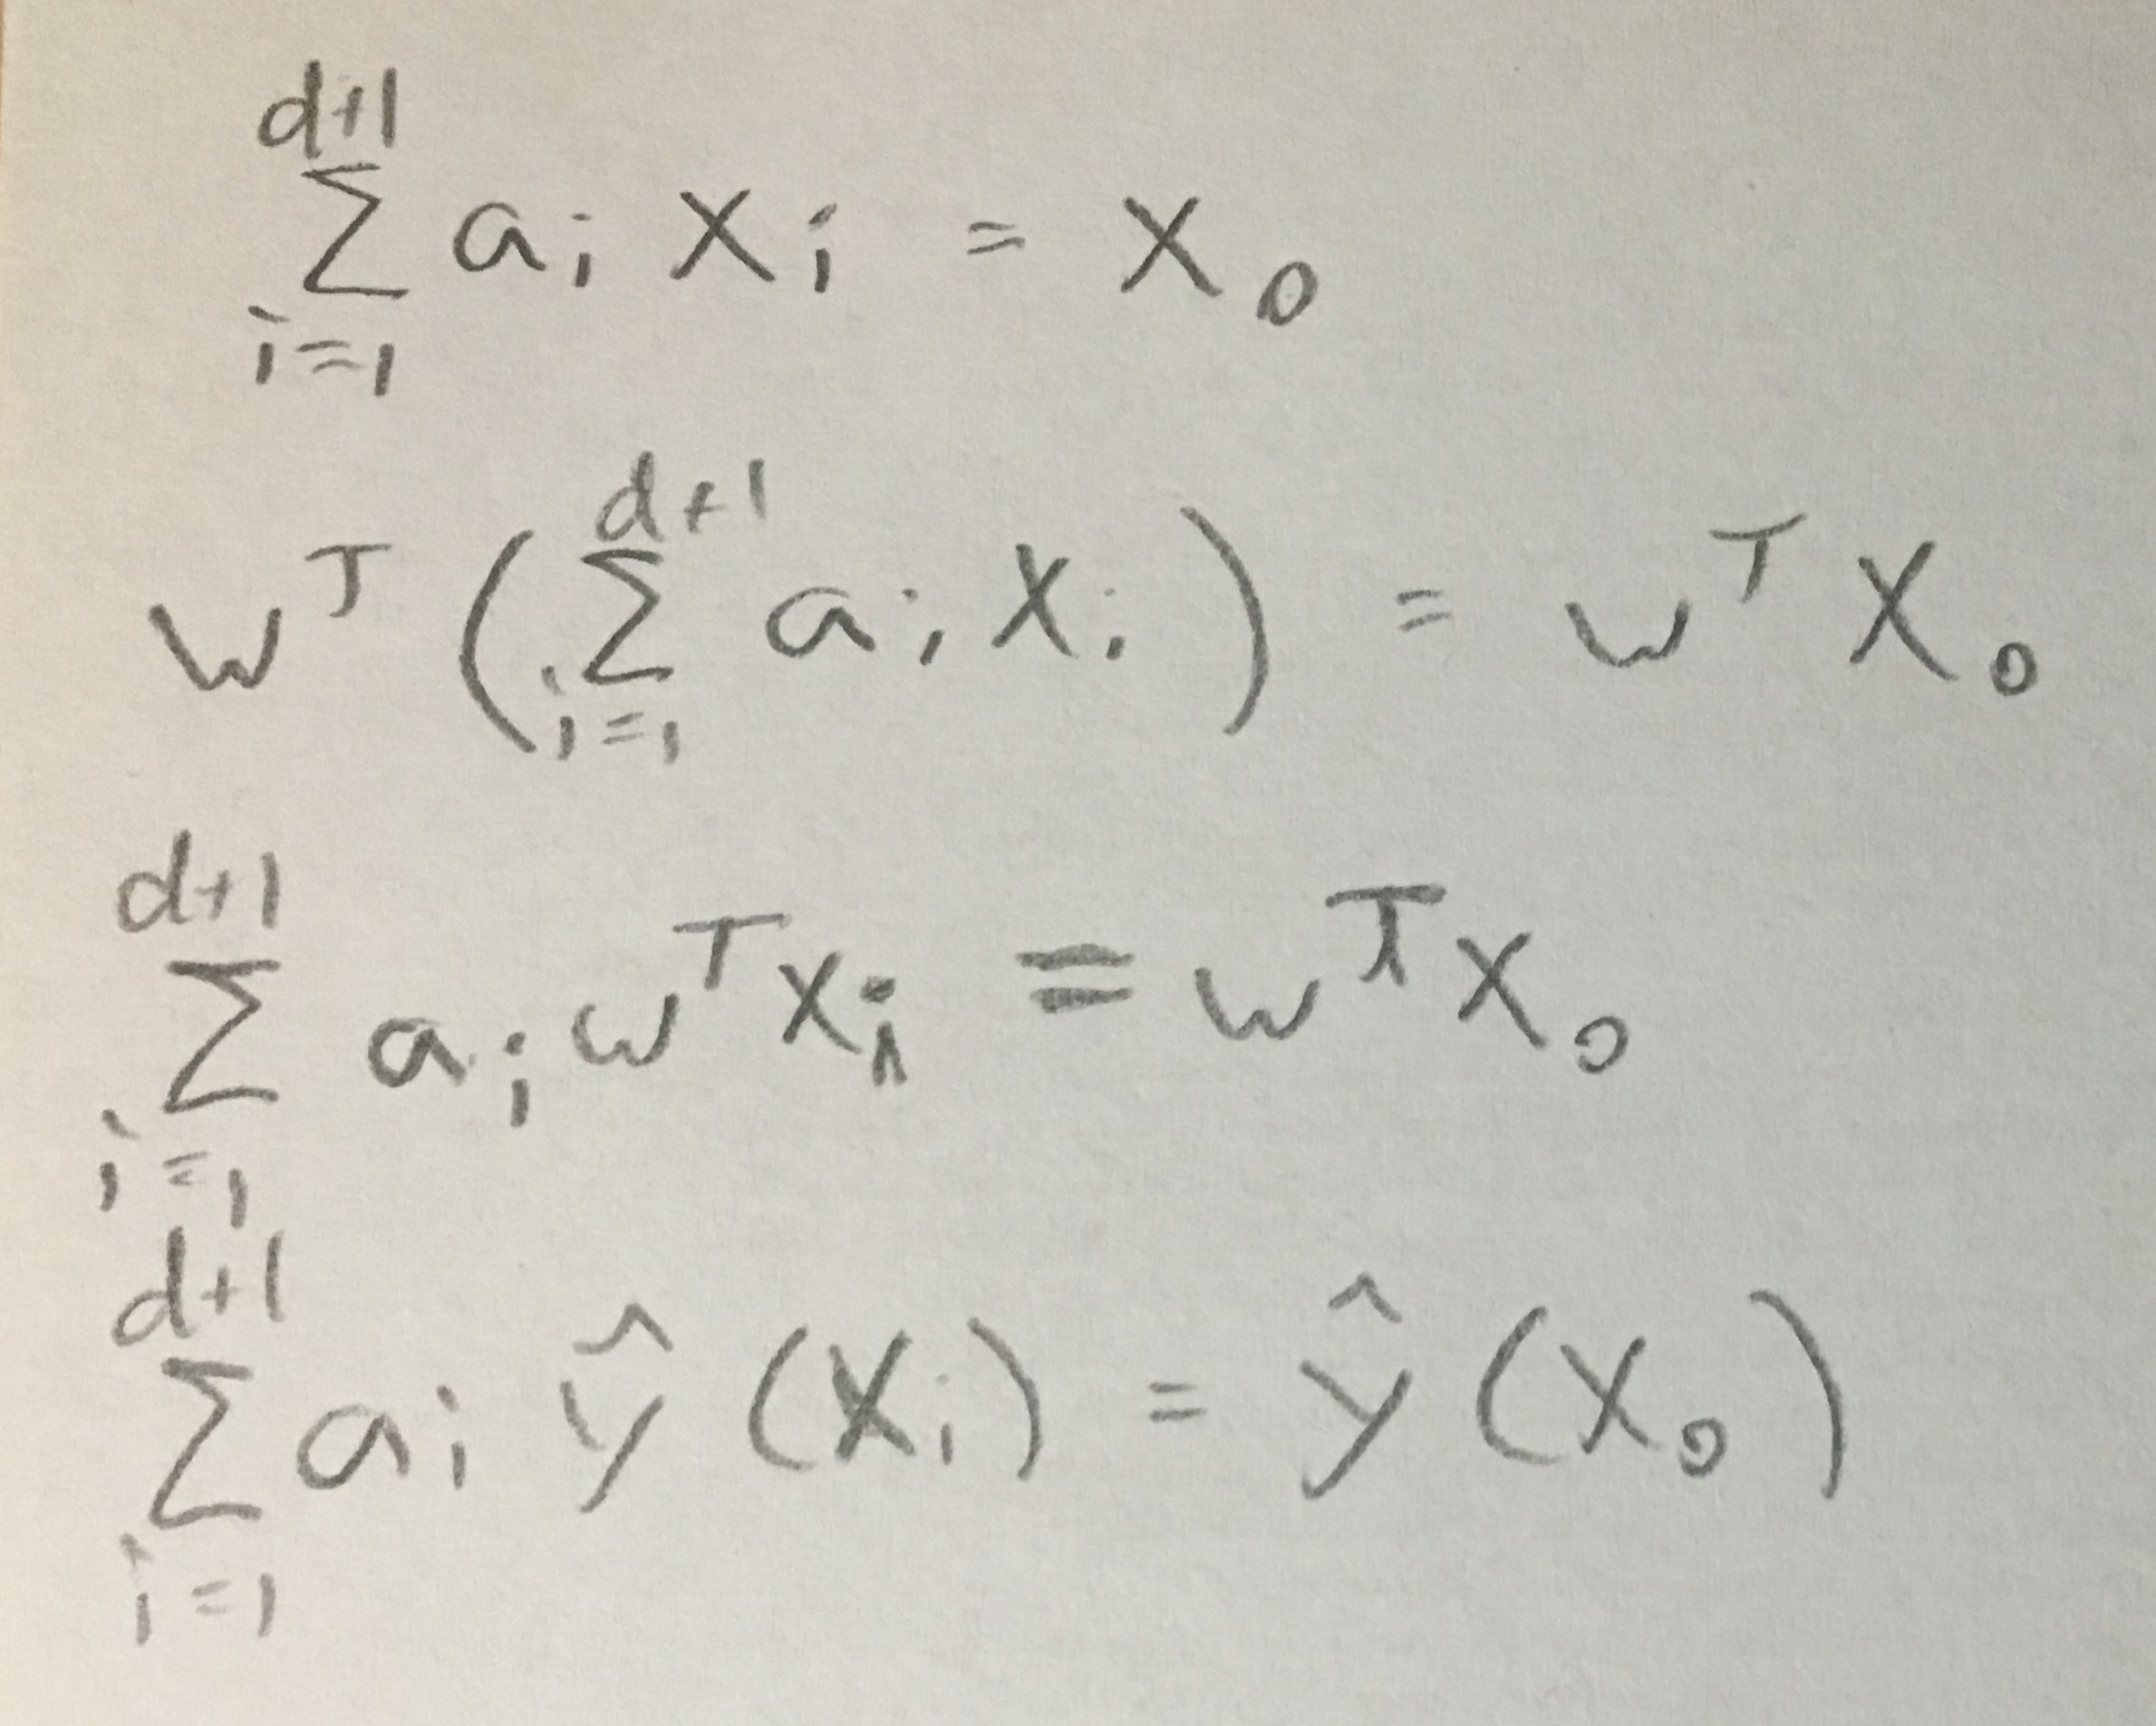
\includegraphics[scale=.1]{IMG_3685.JPG}\\
This means that there will always be one vector whose classification cannot respond to its label, meaning that the set of d+1 vectors cannot be shattered. Thus VC $<$ d + 1. In conjunction with part a, this proves that VC = d. 
\end{enumerate}
\item
\begin{enumerate}
\item If we tried to maximize the cross entropy L(w) on a two class linearly separable data set, we would end up with a runaway parameter w since the maximum possible value of L(w) is zero, but only approaches this asymptotically. This is because a sigmoid function asymptotically approaches 1 from the bottom, thus the log of this function asymptotically approaches 0 from the bottom (and goes to negative infinity in the other direction as the sigmoid goes to zero in that direction) as we can see in the generalized plot of the log of a sigmoid function. \\
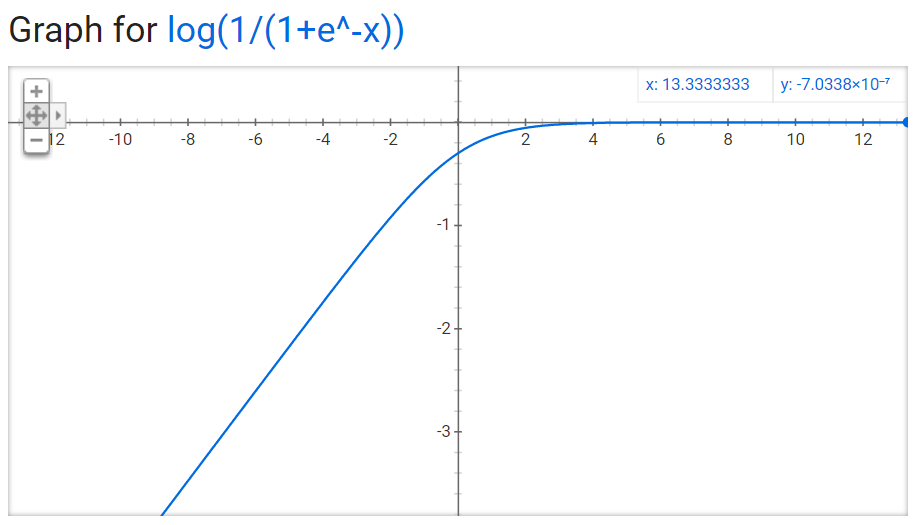
\includegraphics[scale=.9]{sigmoid_graph.PNG}
\\
Once we remove terms corresponding to where yi = 0 or 1-yi = 0 we are left with a sum of the log-of-sigmoid functions: \\
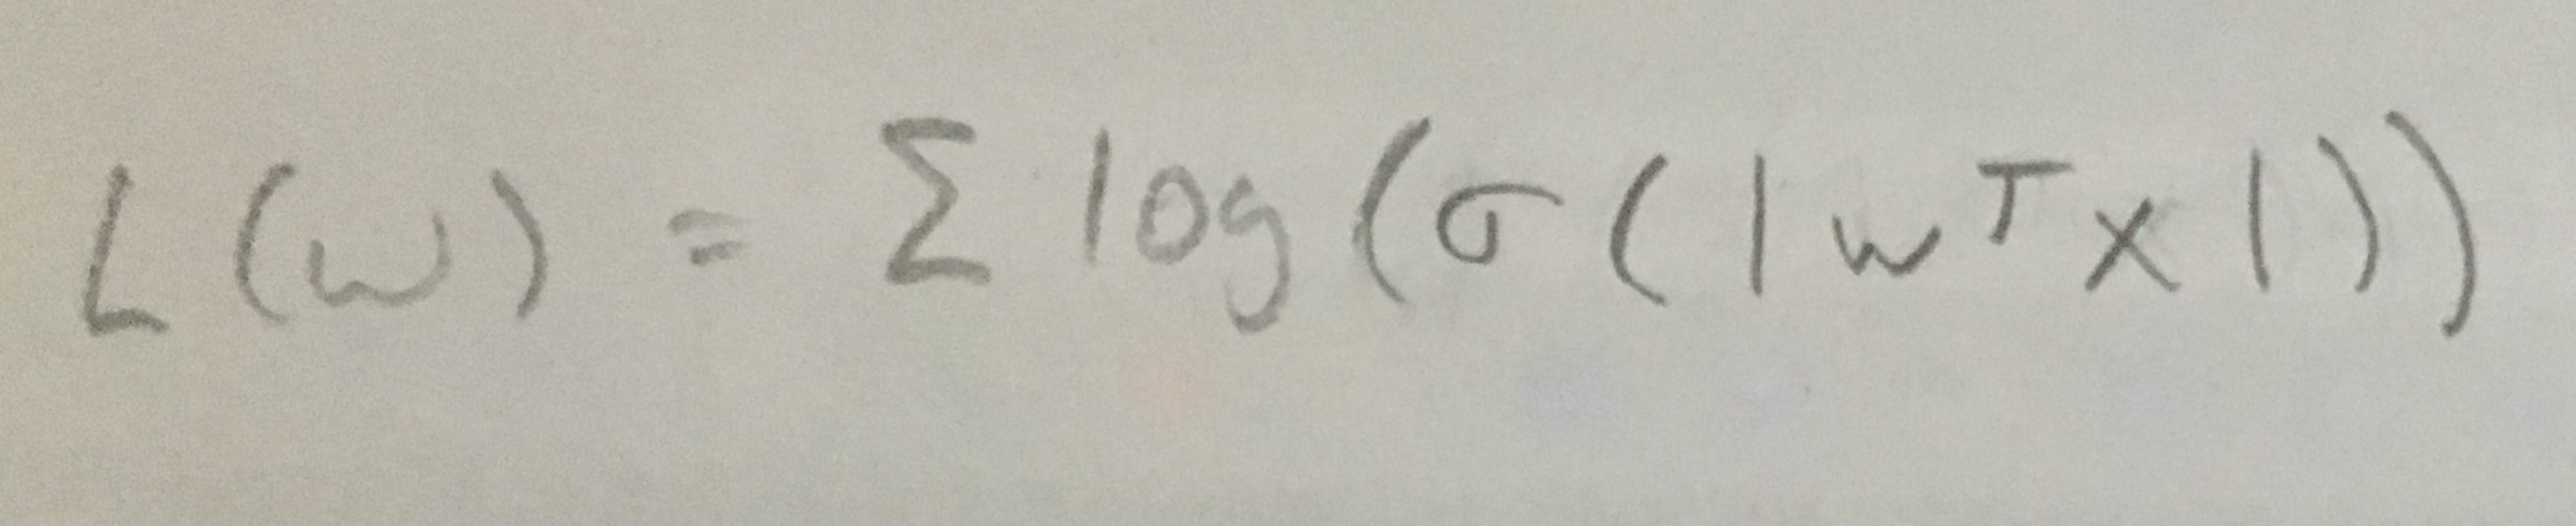
\includegraphics[scale=.1]{IMG_3686.JPG}\\
This implies that the loss function will approach zero in the same way that these component functions do. This means that the arguments to the sigmoid functions, $w^Tx_i$,  will monotonically increase, and since the test points cannot change the hyperplane normal will be forced to increase these products by more and more, driving the components of w to be larger and larger. 
\end{enumerate}
\item 
\begin{enumerate} 
\item A gradient descent step for the squared loss function on two class linear regression can be derived easily by using the fact that the derivative of a sigmoid function is the sigmoid times one minus the sigmoid: \\
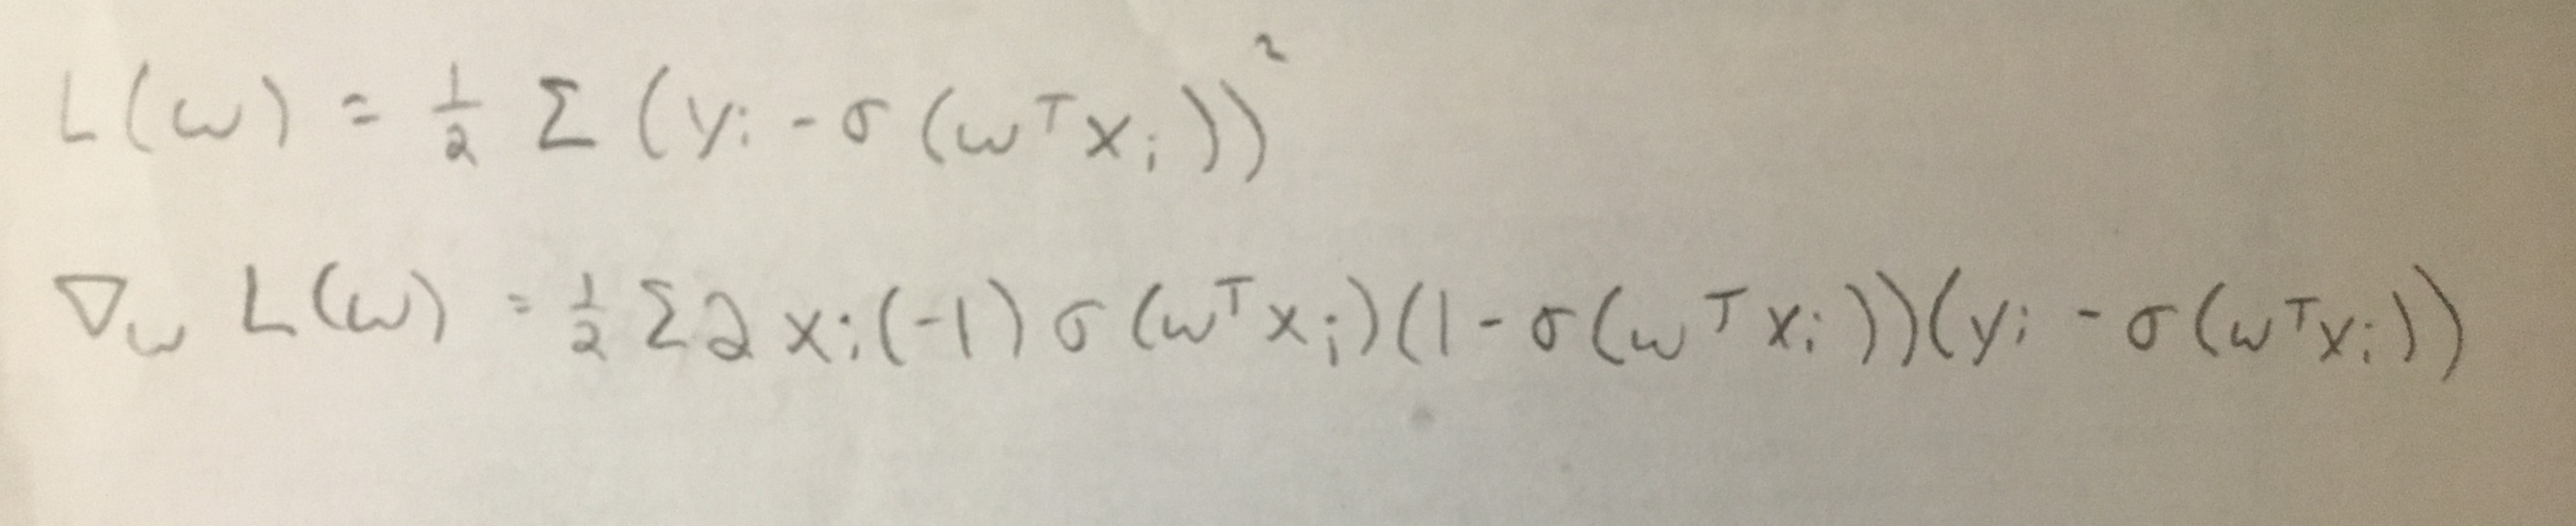
\includegraphics[scale=.05]{IMG_3687.JPG}\\

\item I think that gradient descent for minimizing the squared loss of a linear regression problem is not a bad approach if done well. By that, I mean that the objective function cannot be minimized analytically due to the fact that it only asymptotically approaches its lower bound of zero. Thus gradient descent will also result in a fruitless search for the function's minimum, but we can use it intelligently he must keep track of how much it shifts the loss function by each time. We see the plot of the gradient along one dimension of w below:\\
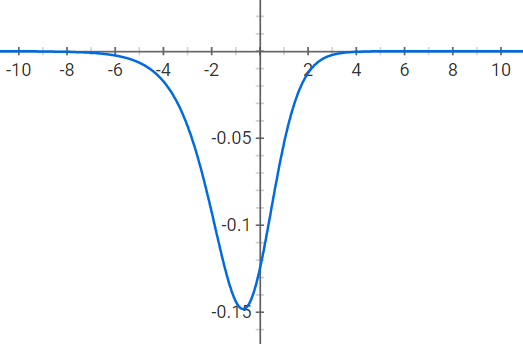
\includegraphics[scale=.8]{23b.PNG}
\\
Once the rate of change is decreasing and has also dropped below a certain threshold, we can be sure that the loss has approached its lower bound (I add the condition that the rate of change is not only below a certain level but also decreasing because if the loss were near its maximum then can see that the rate of change would also be very small, but increasing. This poses another potential flaw in the objective function: if we happen to land on a plane vector which has the loss start very high then it could take a while to optimize the objective, meaning we should start with a few different random w's to reduce the expected run time of the optimization). 
\end{enumerate}

\end{enumerate}




\section{Part 3}

The task here was to implement an Support Vector Machine model with soft margins class. Because the primal objective function for an SVM with soft boundaries is complex and restricted to finite and simple feature vectors, the SVM was trained on the duel of the primal function. This allowed for the potential of complex kernels (ie feature vectors with infinite dimensionality) using the kernel trick, which you will see allowed for much more flexible classification than the linear feature vectors could achieve. \\
To accomplish this, first understand that an SVM attempts to classify points according to the learned predictor \\
$y(x) = w^T\phi(x) + w_0$\\
This predictor is learned by minimizing the primal objective function $L$, which attempts to optimize $w$ and $w_0$ by minimizing the penalty incurred by hinge loss \\
$l_h(x_n, t_n) = max(1 - t_n(w^T\phi(x_n) + w_0), 0)$\\
and in turn maximizing the margin, defined as $\frac{1}{|w|}$\\
To do this, we use the SVM objective function: \\
\\
$L_p = \frac{1}{2}|w|^2 + C \sum_n \zeta_n - \sum_n a_n(t_n(w^T\phi(x_n) - w_0) - 1 - \zeta_n) - \sum_n \mu_n\zeta_n$\\
$w$: the prediction boundary plane \\
$w_0$: the prediction boundary offset\\
$x_n$: the $n^{th}$ training point \\
$t_n$: the $n^{th}$ training label \\
$\zeta_n$: the $n^{th}$ error term proportionate to a point's distance outside its class's margin\\
$a_n$: the $n^{th}$ Lagrange multiplier the hinge loss\\
$\mu_n$: the $n^{th}$ Lagrange multiplier for the $n^{th}$ error term\\
\\
$L_p$ uses the L2 regularizer $|w|^2$ - the square of the norm of the linear separator, the minimization of which pushes the margin to be larger. For data not easily linearly separated, this term alone will cause $w$ to severely over fit the training data to accommodate the distribution. For data which is not linearly separable, this term alone will cause the objective function to be unsolvable. \\
This is why we also use the inverse regulator $C$ in $C \sum_n \zeta_n$. By allowing for these error terms, we make it possible to solve the objective function on data which is not linearly separable. However, we want to minimize this error, so we take the sum of the error terms, multiply by $C$, and add this to $L$ to be minimized as well, thus instilling an inherent trade-off between maximizing the size of the margin and minimizing the misclassification.\\
To simplify the problem and allow for a more flexible objective function, I defined the duel objective function: \\
$L_d = q^Ta + \frac{1}{2}a^TPa$\\
$q$: the length $N$ vector of $-1$'s\\
$P$: was the gram matrix $K = \Phi\Phi^T$ multiplied element wise by  the outer product of the labels $t$ so $P = \Phi\Phi^T .* tt^T$\\
This objective function needed to be minimized subject to the constraints \\
$0 \leq a_n \leq C$ (Lagrange multipliers are between $0$ and $C$)\\
$t^Ta = 0$ (the sum of the labels weighted by the Lagrange multipliers was zero)\\
By the quadratic convex nature of the Lagrange objective function $L_d$ and the constraints placed upon it, I knew minimizing it found its one and only local minimum and thus its global minimum. This meant I could explore minimization strategies beyond gradient descent. Here a quadratic optimizer from the cvxopt library was used to find the optimal $a$ vector. 
Because this was the duel objective of the primal objective which sought to find an optimal $w$, $w_0$, and $\set(\zeta_n)$, finding the optimal values for $a$ also found the optimal values for $w$, $w_0$ but while allowing for the usage of a kernel matrix in place of more restrictive feature vectors. This means we can then classify test points and build visualizations of the model's predictions of the underlying class distributions. \\
 
\begin{wrapfigure}{r}{0.5\textwidth} %this figure will be at the right
    \centering
    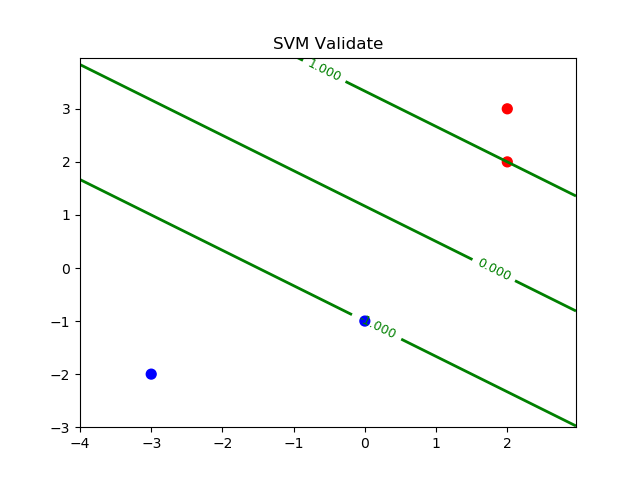
\includegraphics[width=0.5\textwidth]{mini_batch.png}
\end{wrapfigure}

In the simple test example with four points, with red as positive and blue as negative, we see that $(2, 2)$ is a the support vector for the positive boundary and $(0, -1)$ is the support vector for the negative boundary. \\
In figure 1 we see that with larger, more complex data sets, that the linear classifier is only sometimes able to achieve comparably clean results. When using C=1, we see that in the datasets on the left are relatively well separated. For dataset 1 we have w = [-0.18297829,  1.76127962] and this perfectly separated the data, but due to the inverse regularization from the C term not all points are within their boundaries however. The line over dataset 3 with w = [-0.04753449,  3.43177734] does misclassify some points (error rate of 0.02) but does rather well due to the very separate class distributions. Datasets 2 and 4 are different, however. Dataset 2 has strongly overlapping and nonlinear class distributions, thus the linear classifier w = [ 1.31477194, -0.04219494] manages only to separate the general centers of the shapes, resulting in an error rate of .17. Dataset 4 is clearly an Xor collection of data, a canonically non linearly separable shape, thus the linear separator w = [-0.21860975, -0.21106405] again fails with an error rate of .3, despite very separate class distributions.\\

Once we moved on to a more complex kernel, in this case the gaussian kernel where $k(x, x') = e^{-\gamma \abs(x - x')}$, we entered into an infinite dimensional feature space, one which could conform to the irregular and nonlinear, even separated, shapes of difficult to fit datasets. In Figure 2, we see how with the same C=1, we were able to significantly reduce the error rates in the second dataset (0.06) and the fourth dataset (0.0325). The first and third datasets are not shown because the linear classifier already performed well on them, thus the Gaussian kernel could not yield much improvement and was therefore uninteresting in those contexts. \\
With multiple kernels and datasets it became possible to investigate interesting trends between variables such as margin, C, bandwidth, kernel, and accuracy. See these in Figure 3\\
We see in Figure 3a that, as we expect, the margin decreases as C is increased. This is because having a higher C penalizes the errors more strongly, thus pushing the margin to more tightly conform to the data. The end result is a margin which is necessarily smaller to accommodate this more intricate shape. Looking over the differences between the datasets we observe the dataset 4 is a clear outlier. Since XOR is a very separable (though not linearly) dataset, it was easily classified with high integrity but also a large margin. Among the other datasets, we observe that dataset two appears to have reached its asymptotic (as C goes to infinity) margin most quickly. This is likely because the class distributions overlap so much that no margin can classify them well, thus penalizing the errors more strictly cannot force the classifier into a more discriminating shape and thus the margin stays the same. datasets 1 and 3 you'll recall are the most linearly separable. This is why we observe them reaching their asymptotic margins last; they have a lot of room between the decision plane and the bulk of the data so the margin can shrink or expand depending on how strongly the points outside of it are penalized. The margin will always be weakly decreasing as a function C since increasing C can only ever serve to increase the penalty of errors, which can never cause the margin to increase since that would also increase the aggregate error.\\
In figures 2a and 2b we observe the dependence of the number of support vectors (vectors on or outside the margin) on C, the penalty on errors. At  high level, it is easy to see the two are inversely correlated. This makes sense, as C increases we would expect the model to penalize points outside the margin more, thus resulting in fewer of them, meaning fewer support vectors. Dataset 4 with the linear kernel is an interesting case because the number of support vectors seems to be constant and saturated at almost 400 (nearly all of them). We could have guessed this from Figure 1d where the plot shows that, while most of the data is classified correctly, only a tiny portion is actually behind the correct class margin. This means almost all the data are support vectors. This cannot change regardless of C because this data is inherently inseparable by a linear classifier. Similarly predictable, we observe that the linear classifier could not manage to reduce the number of support vectors far below 200 for the second data set, also due to its inherent inseparability (especially by a linear classifier). Meanwhile we see that the Gaussian kernel exhibited much stronger correlations between the number of support vectors and C. This is because, in conforming more complexly to the data distributions, the classifier is able to build up a larger margin, which in turn as more room to shrink as the errors are more strongly penalized. \\ 
Maximizing the margin may not be the right way to choose C because increasing the margin may seem to make the inferred class distributions more general and resistant to over fitting but this may not always be the case. Like with any trade off, there is a balancing point. If we take this to its extreme we could let C=0, allowing for a very large margin, but without penalty for misclassified points. This means that we certainly don't have to worry about our model being too sensitive to training data but we do have to worry about it not being sensitive enough. A better way to choose an ideal C is to train it as a hyperparameter on test data before finally evaluating the final model on the validation data.\\
\begin{figure}
  \centering
  \caption{\label{Data }Linear Kernal}
  \subfloat[Dataset1]{\label{data1}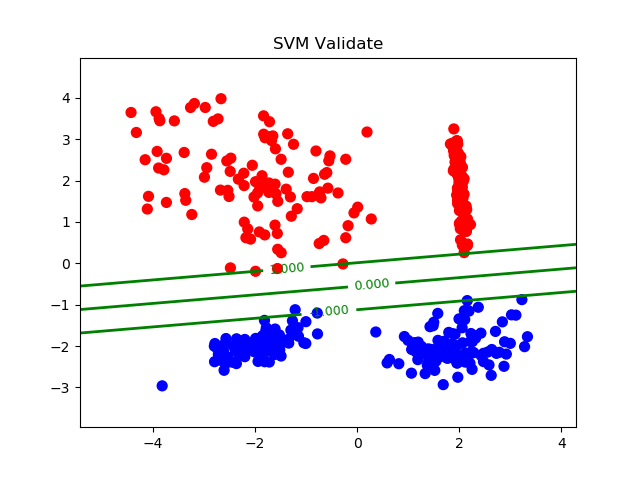
\includegraphics[width=0.5\textwidth]{part2_linear_1.png}}
  \subfloat[Dataset2]{\label{data2}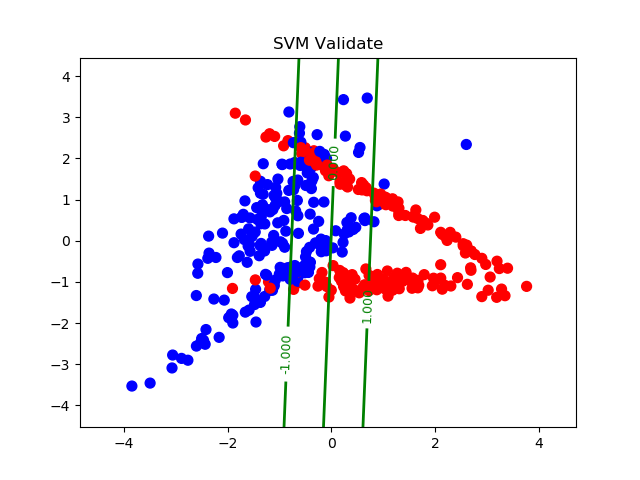
\includegraphics[width=0.5\textwidth]{part2_linear_2.png}}
  \newline
  \subfloat[Dataset3]{\label{data3}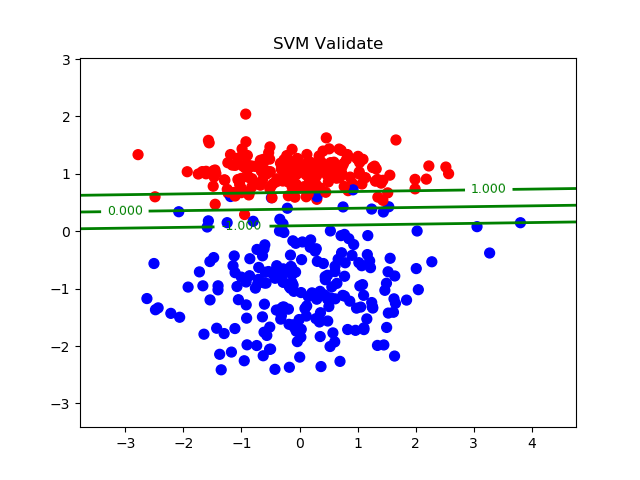
\includegraphics[width=0.5\textwidth]{part2_linear_3.png}}
  \subfloat[Dataset4]{\label{data4}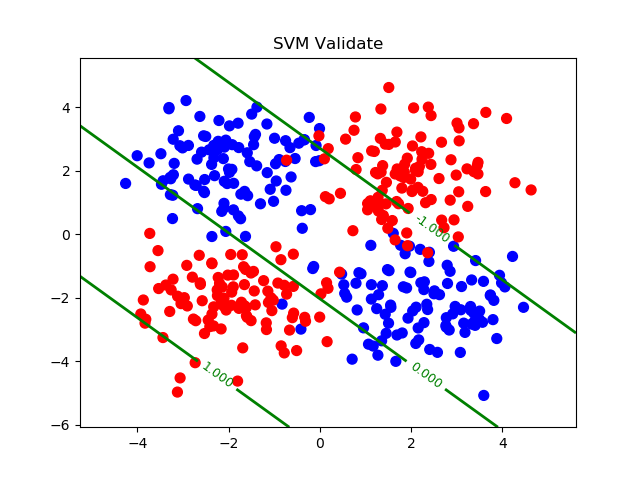
\includegraphics[width=0.5\textwidth]{part2_linear_4.png}}
   \newline
  \caption{\label{Data }Gaussian Kernal}
  \subfloat[Dataset2]{\label{data12}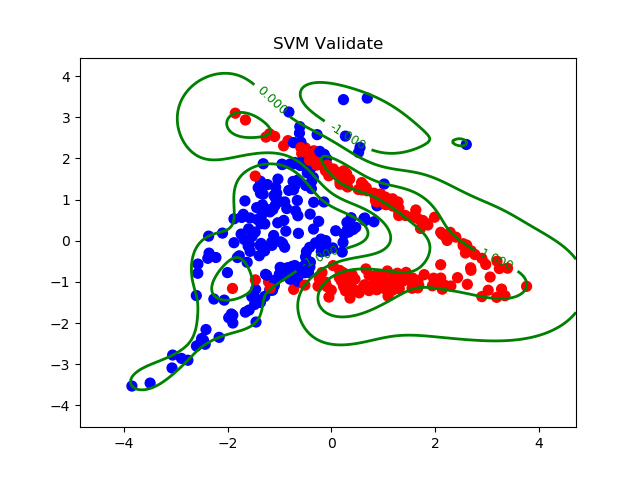
\includegraphics[width=0.5\textwidth]{part2_gauss_2.png}}
  \subfloat[Dataset4]{\label{data42}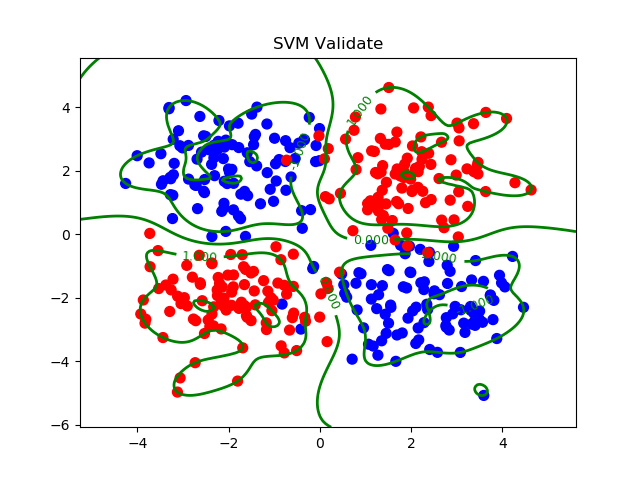
\includegraphics[width=0.5\textwidth]{part2_gauss_4.png}}
\end{figure}

\begin{figure}
  \centering
  \caption{\label{Data }Trends Investigated}
  \subfloat[]{\label{data5}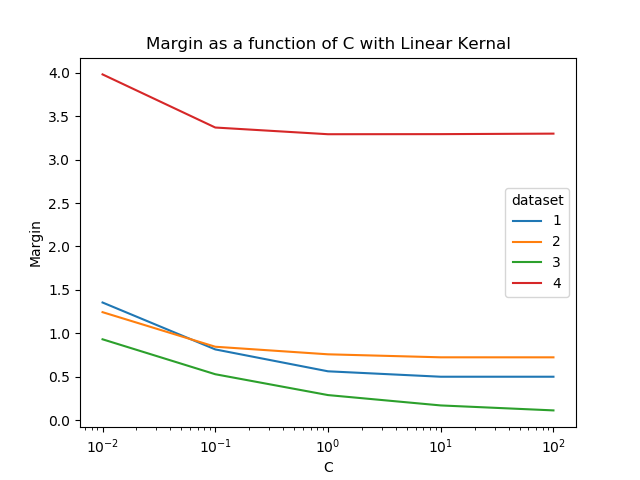
\includegraphics[width=0.5\textwidth]{margin_vs_C_linear.png}}
  \newline
  \subfloat[]{\label{data7}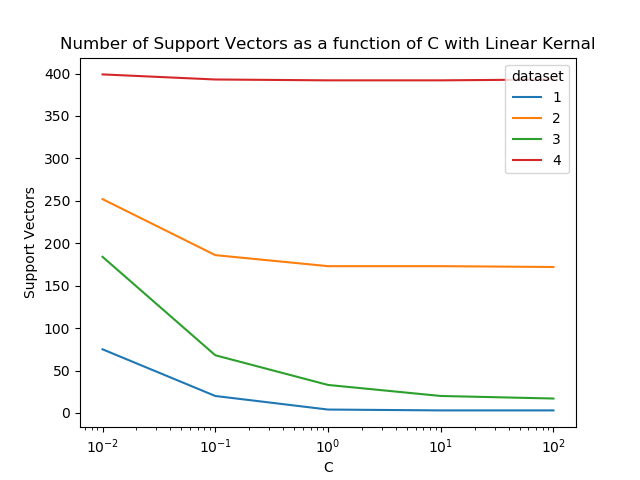
\includegraphics[width=0.5\textwidth]{support_vecs_vs_c_linear.png}}
  \subfloat[]{\label{data8}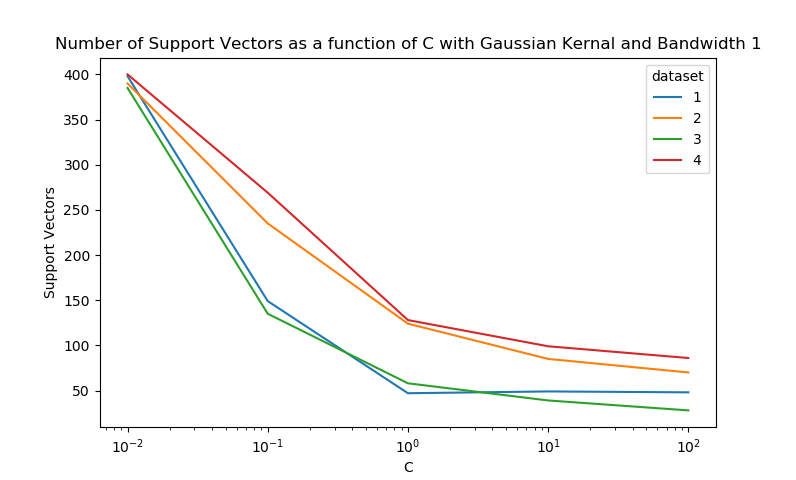
\includegraphics[width=0.5\textwidth]{support_vecs_vs_c_gauss.png}}
\end{figure}

\newpage

\end{document}
